\documentclass[10pt,letterpaper]{article}
\usepackage[top=0.85in,left=2.75in,footskip=0.75in]{geometry}
\usepackage{bibentry}

% Text layout specific to Supplemental Materials
\topmargin 0.0cm
\oddsidemargin 0.5cm
\evensidemargin 0.5cm
\textwidth 16cm
\textheight 21cm

\setlength{\parskip}{1em}

% Template for PLoS
% Version 3.2 March 2016

% General commands for text/figures

% Page margin
\usepackage[top=0.85in,left=2.75in,footskip=0.75in]{geometry}
% Use Unicode characters when possible
\usepackage[utf8x]{inputenc}
% amsmath package, useful for mathematical formulas
\usepackage{amsmath}
%\usepackage{natbib}
% amssymb package, useful for mathematical symbols
\usepackage{amssymb}
%\usepackage{booktabs}
\usepackage{xspace}
\usepackage{hyperref}
% graphicx package, useful for including eps and pdf graphics
% include graphics with the command \includegraphics
\usepackage{graphicx}

% Use adjustwidth environment to exceed column width (see example table in text)
\usepackage{changepage}

% textcomp package and marvosym package for additional characters
\usepackage{textcomp,marvosym}

% fixltx2e package for \textsubscript
\usepackage{fixltx2e}

% cite package, to clean up citations in the main text. Do not remove.
\usepackage{cite}
\usepackage{caption}
\usepackage{subcaption}
\usepackage{rotating}

\usepackage{color}

% Use doublespacing - comment out for single spacing
%\usepackage{setspace}
%\doublespacing


% Bold the 'Figure #' in the caption and separate it with a period
% Captions will be left justified
\usepackage[labelfont=bf,labelsep=period,justification=raggedright]{caption}

% Use the PLoS provided bibtex style
%\bibliographystyle{/Users/stephens/Dropbox/Documents/stylefiles/plos2009}

% Remove brackets from numbering in List of References
\makeatletter
\renewcommand{\@biblabel}[1]{\quad#1.}
\makeatother

% Use nameref to cite supporting information files (see Supporting Information section for more info)
\usepackage{nameref,hyperref}

% line numbers
%\usepackage[right]{lineno}

% ligatures disabled
\usepackage{microtype}
\DisableLigatures[f]{encoding = *, family = * }

% Leave date blank
\date{}

%\pagestyle{myheadings}
%% ** EDIT HERE **
\usepackage{enumerate}
\usepackage{multirow}
\usepackage{url}
\usepackage{xr} %for cross-referencing
%% ** EDIT HERE **
%% PLEASE INCLUDE ALL MACROS BELOW
\newtheorem{algorithm}{Algorithm}
\newtheorem{proposition}{Proposition}
\newtheorem{restateproposition}{Proposition}
\newtheorem{lemma}{Lemma}
\newtheorem{corollary}{Corollary}
\newtheorem{result}{Result}
\newtheorem{note}{Note}
\newtheorem{definition}{Definition}

\def\KL{\text{KL}}

% Text layout
\raggedright
\setlength{\parindent}{0.5cm}
\textwidth 5.25in
\textheight 8.75in

% Bold the 'Figure #' in the caption and separate it from the title/caption with a period
% Captions will be left justified
\usepackage[aboveskip=1pt,labelfont=bf,labelsep=period,justification=raggedright,singlelinecheck=off]{caption}
\renewcommand{\figurename}{Fig}

%------ bibliography
% Use the PLoS provided BiBTeX style
\bibliographystyle{bmc-mathphys}
% Remove brackets from numbering in List of References
\makeatletter
\renewcommand{\@biblabel}[1]{\quad#1.}
\makeatother


%% Author's settings
\def\KL{\text{KL}}

\pagestyle{empty} %%in order to delete the number at the bottom of the page


\begin{document}

\section*{Figures}
\newpage

\begin{figure*}[h!]
\centering
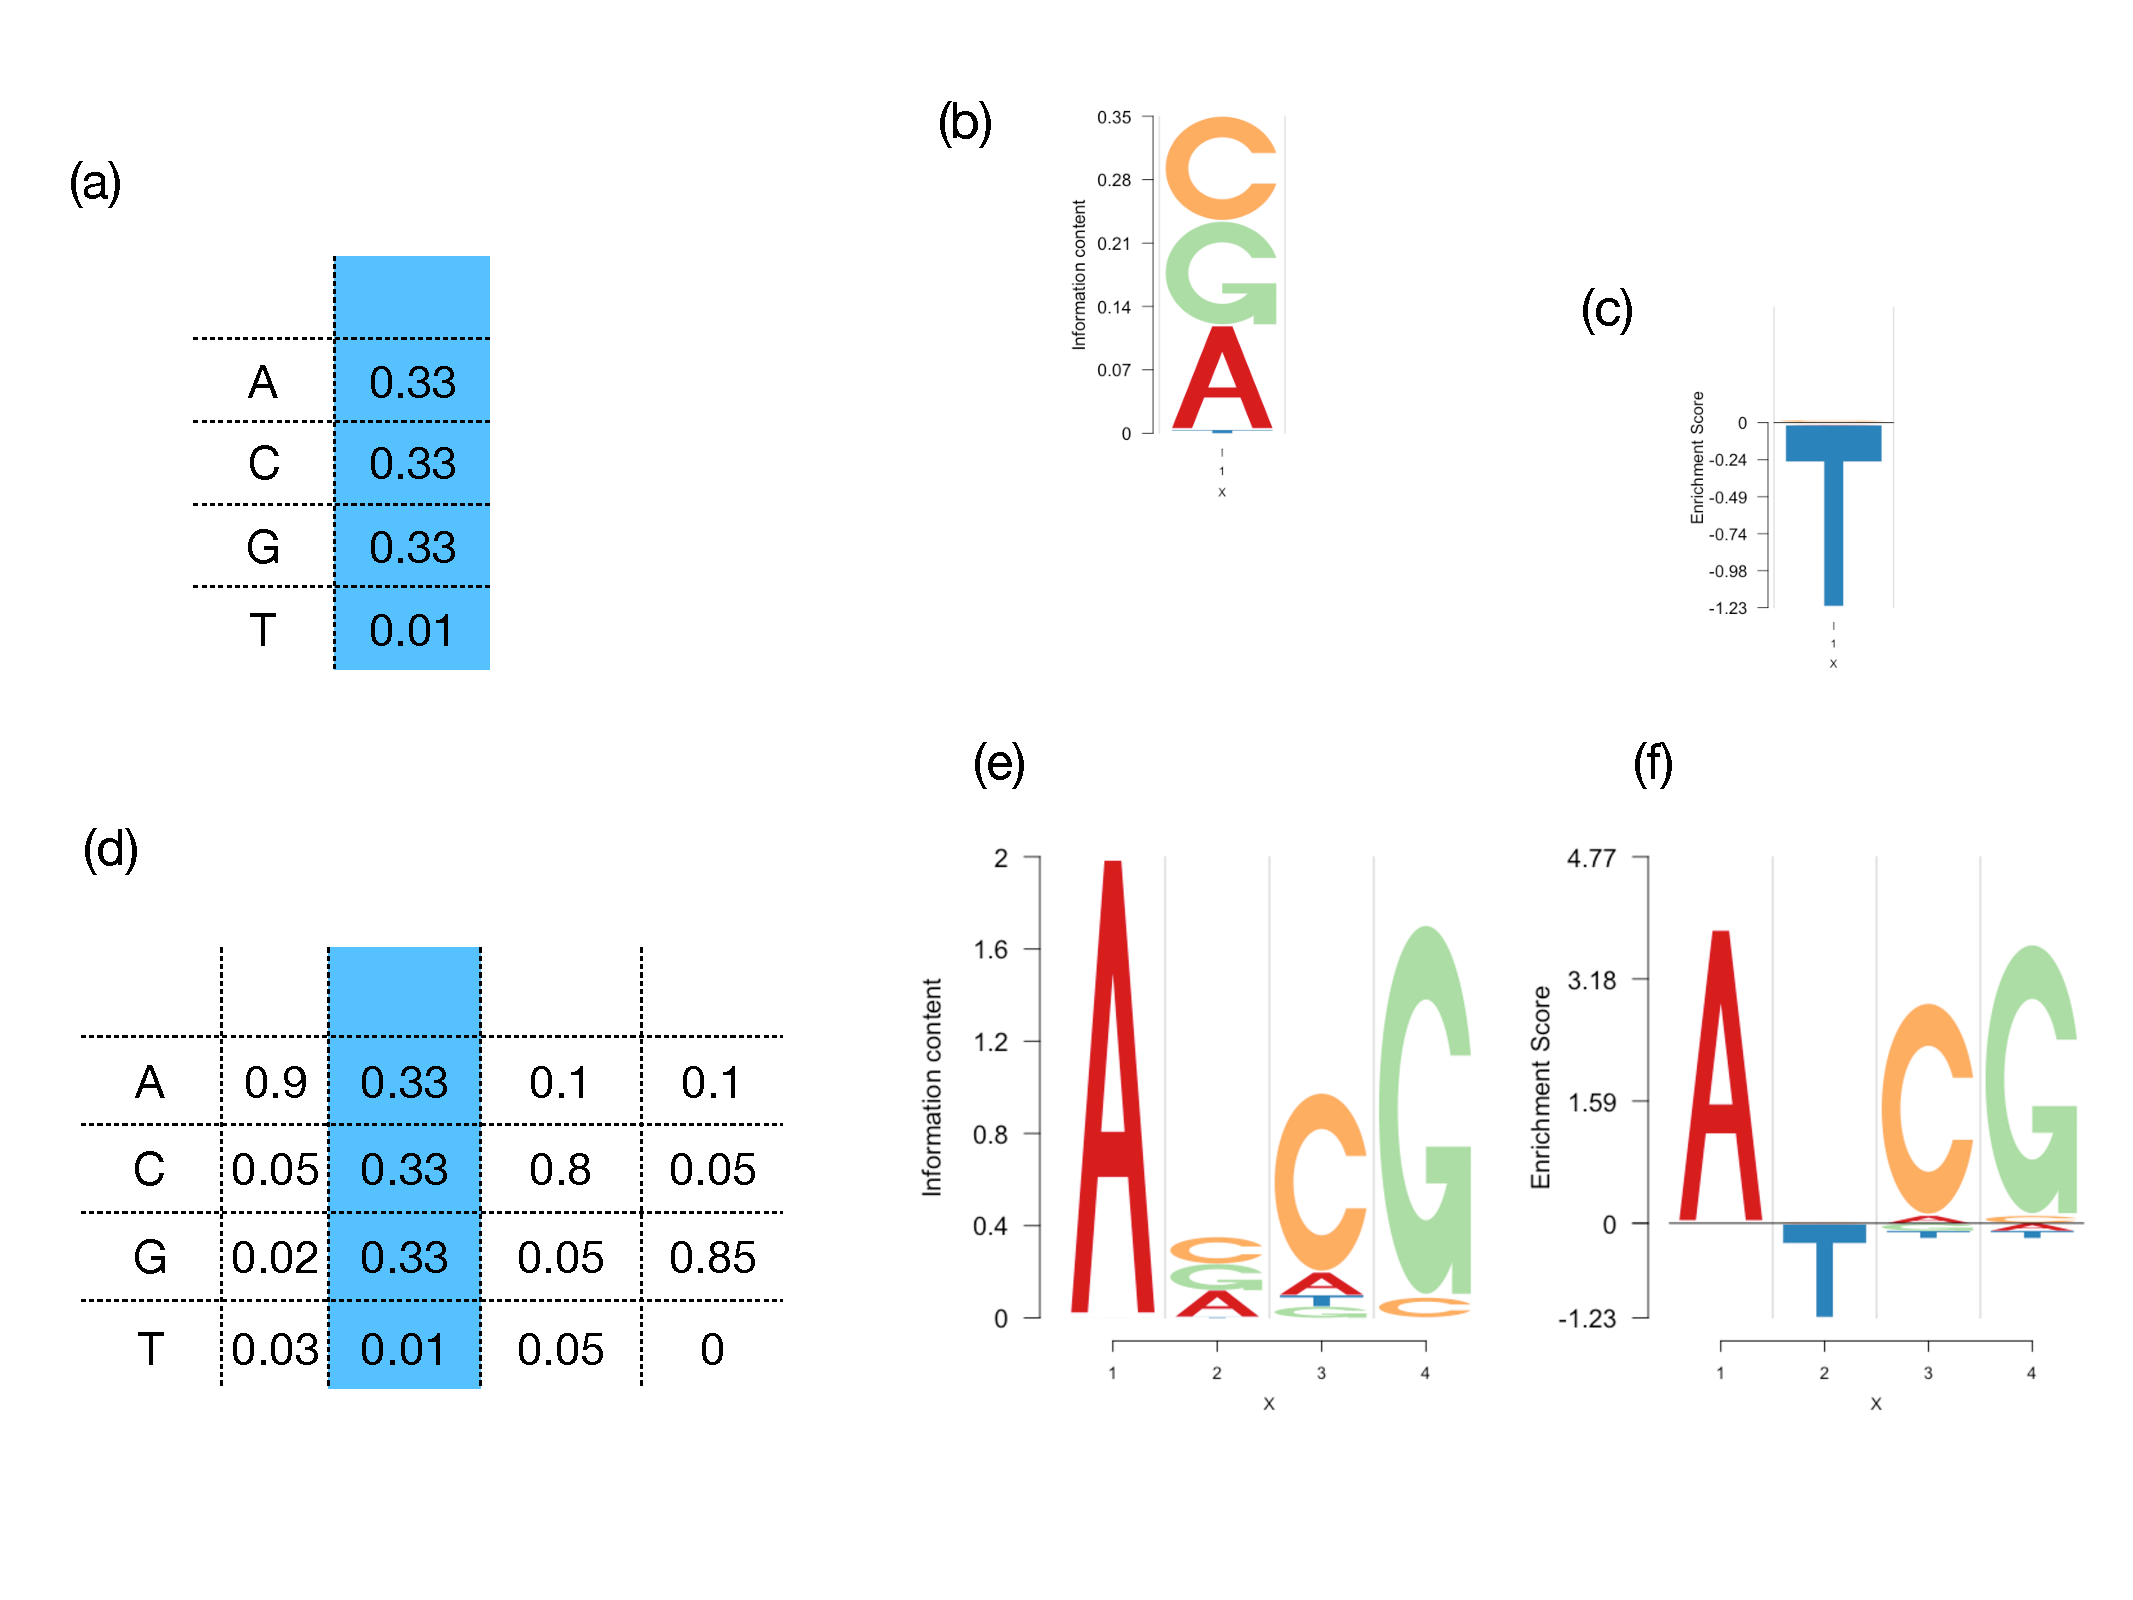
\includegraphics[height=6in, width=7in]{figures_folder/figures16.pdf}
\caption{\textbf{Illustration of the sparse logo representation.}
      We present an illustration of how sparse logo representation accounts for depletion signal and provides a more informative visualization of the sequence motif. In panel (a), we present a positional weight vector with a depletion of the base $T$ while the other bases have similar position weights. In panel (b), we present the standard logo representation of this positional vector that highlights the abundance of $A$, $C$ and $G$ at this position. In panel (c), we present the sparse logo representation (ratio approach) that highlights the depletion of $T$ instead.  In panel (d), we present a position weight matrix with the position weight  vector in panel (a) at the second position flanked by enrichments around it. In panel (e), we present the corresponding standard logo plot representation of the PWM matrix at panel (d). The signal at the second position gets swamped by the bias towards enrichment signals flanking it. In panel (f), we present the sparse logo representation of the PWM matrix in (d), where both the enrichment signals as well as the depletion signal at position 2 are clearly observed.}
\label{fig:fig1}
\end{figure*}

\begin{figure*}[h!]
\centering
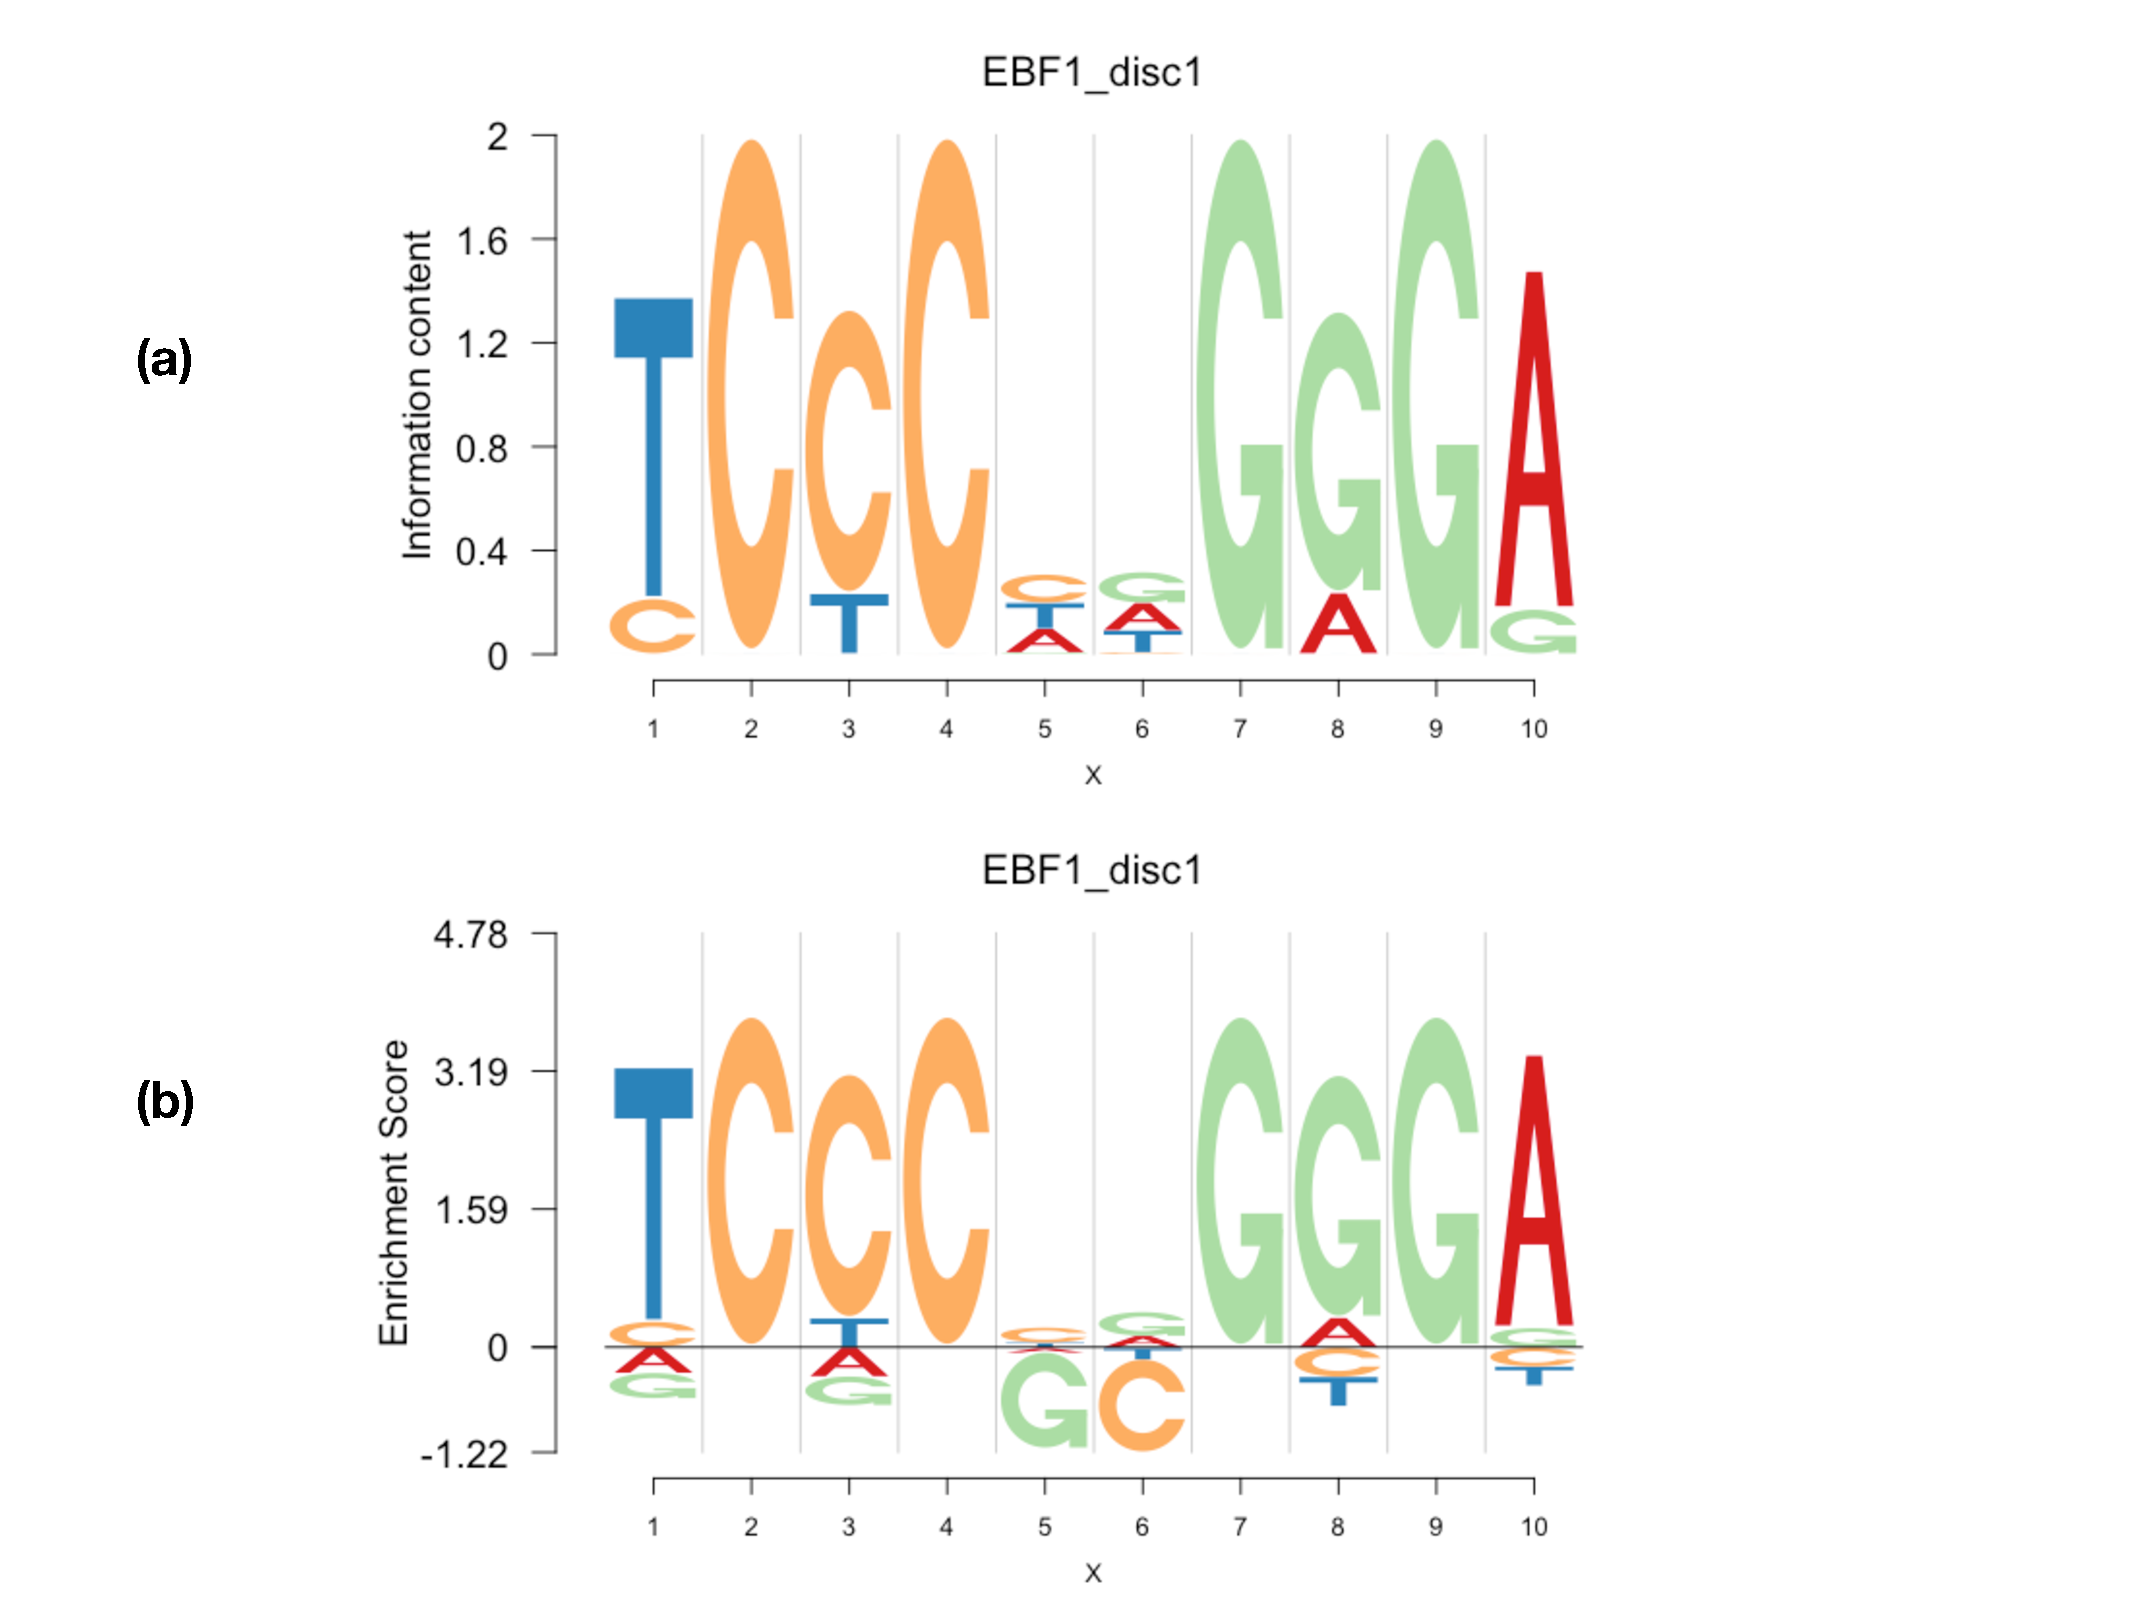
\includegraphics[height=6in, width=7in]{figures_folder/figures5.pdf}
\caption{\textbf{Application of sparse logo in detecting depletion patterns in Transcription Factor Binding sites (TFBS).}
      We present the standard logo and the sparse logo representation of a transcription factor EBF1-disc1. The logo standard logo plot in panel (a) seems to indicate that the transcription factor binds in a dimerized form to its binding site. However, it fails to capture the depletion of G and C in the two positions in the middle of the dimer, which is apparently captured by the sparse logo representation in panel (b). The stack heights in the sparse logo representation in this plot has been determined by the \textit{log} approach. The PWM data for EBF1-disc1, computed from the ENCODE TF Chip-seq datasets, is hosted on the webpage \url{http://compbio.mit.edu/encode-motifs/}\cite{Kheradpour2013}}
\label{fig:fig1}
\end{figure*}

\begin{figure*}[h!]
\centering
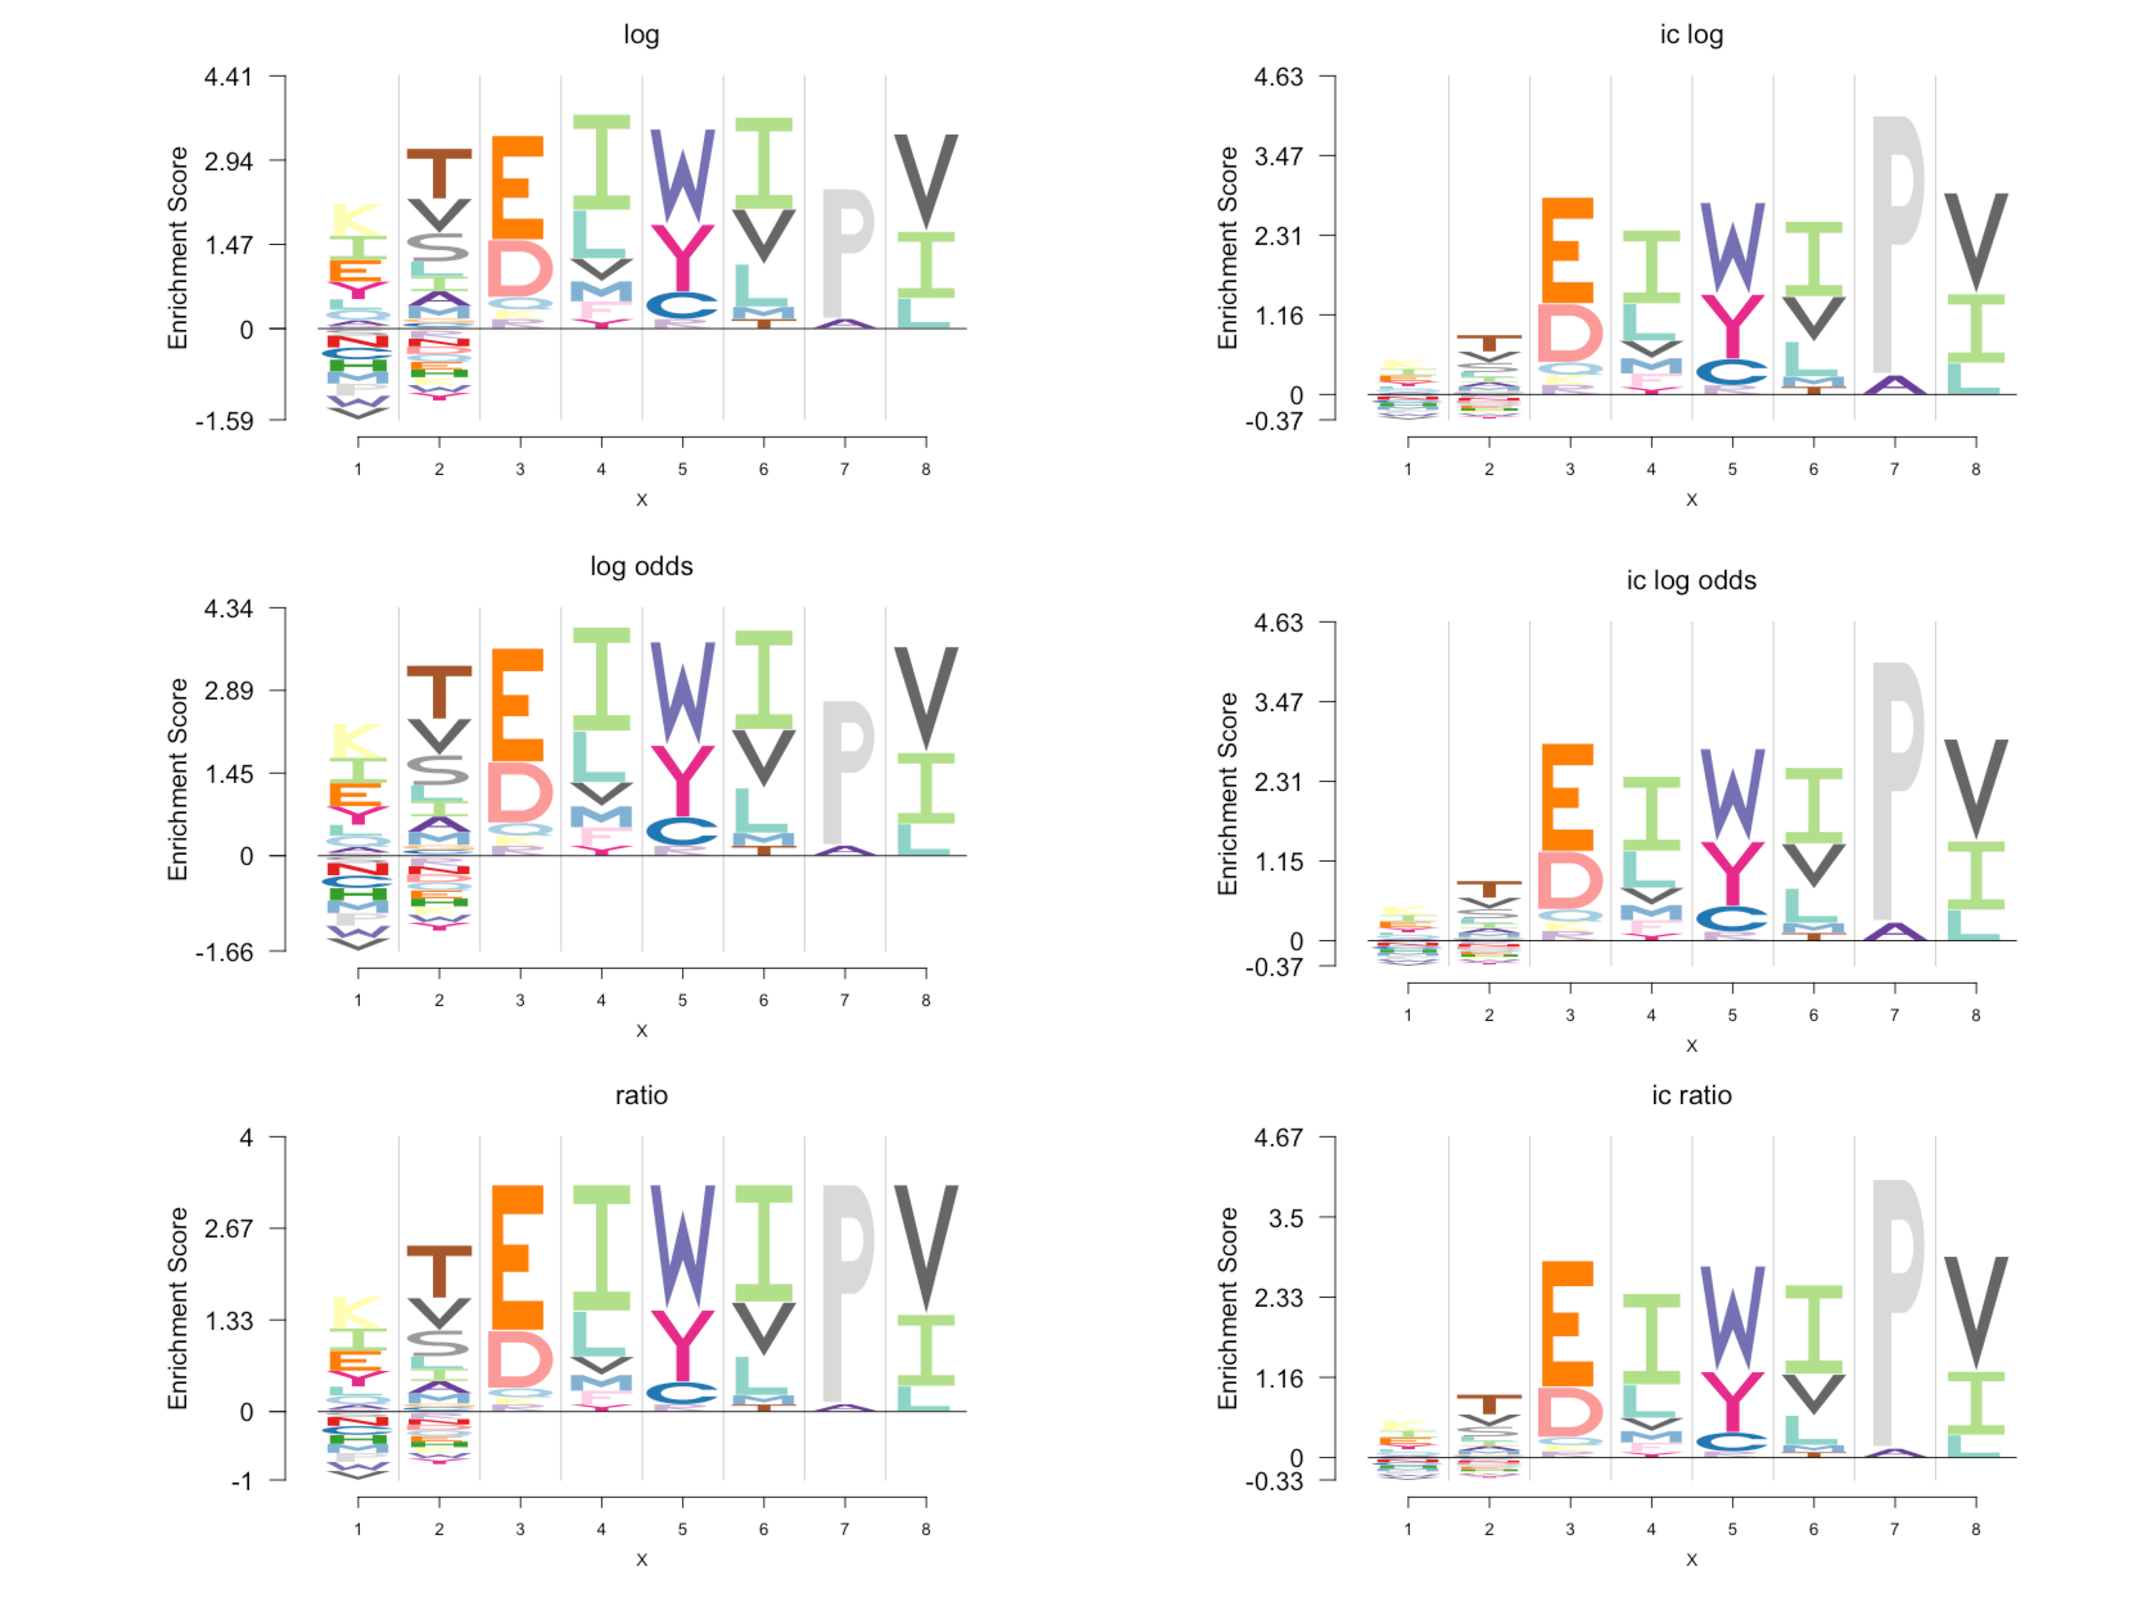
\includegraphics[height=6in, width=7in]{figures_folder/figures7.pdf}
\caption{\textbf{Various sparse logo representations of protein sequence motif.}
 The sparse logo representation under various stack height and stack composition methods - \textit{log}, \textit{log-odds}, \textit{ratio}, \textit{ic-log}, \textit{ic-log-odds} and \textit{ic-ratio} for the Bacterial transcription activator, effector binding domain protein PF06445 (motif 4, Start=153 Length=8). The data is fetched from the 3PFDB website \url{http://caps.ncbs.res.in/cgi-bin/mini/databases/3pfdb/get_entry.cgi?id=PF06445}.}
\label{fig:fig2}
\end{figure*}

\begin{figure*}[h!]
\centering
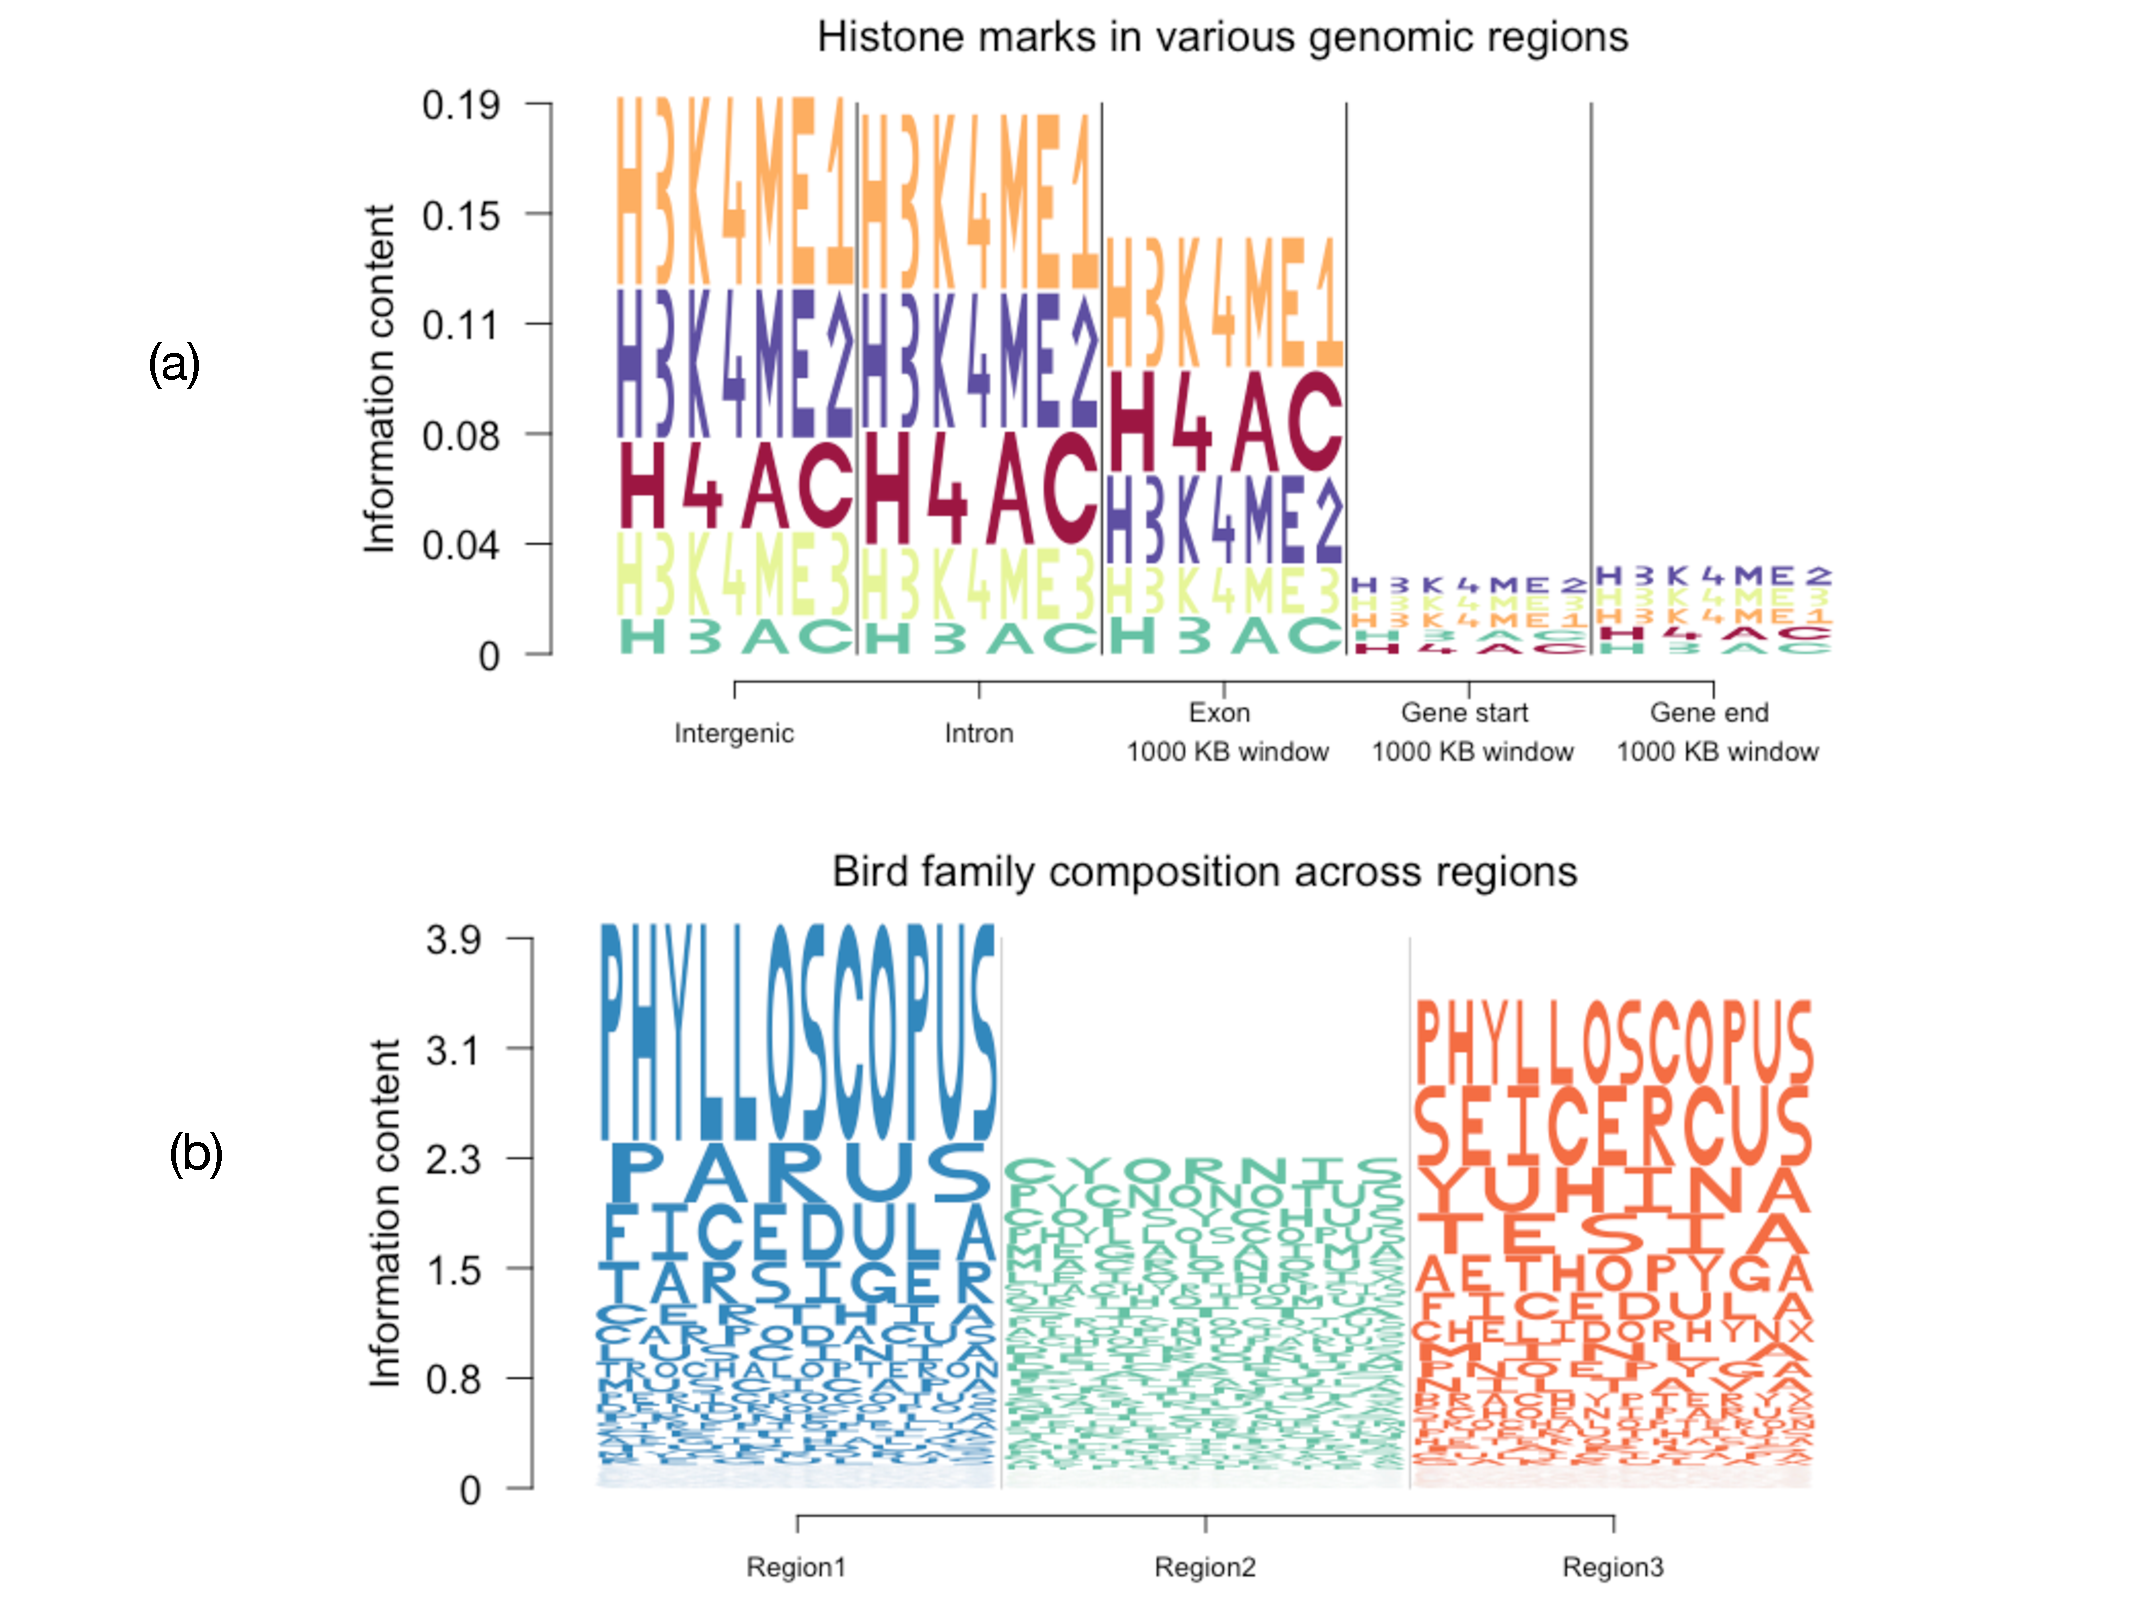
\includegraphics[height=6in, width=7in]{figures_folder/figures3.pdf}
 \caption{\textbf{Example applications of string logo plots.}
      We present two example biological applications of string logo plots.
In panel (a), we present the logo plot representation of the composition of histone modification types that overlap with an intergenic region, intron, exon, gene start or gene end for the lymphoblastoid cell line GM06990 as reported in Koch et al 2007 \cite{Koch2007}. In panel (b), we present the logo plot representation of the abundance compositions of bird species  families in three different regions of the Himalayas - colored red, green and blue. The data has been taken from White et al 2017 [ref].}
\label{fig:fig3}
\end{figure*}


\begin{figure*}[h!]
\centering
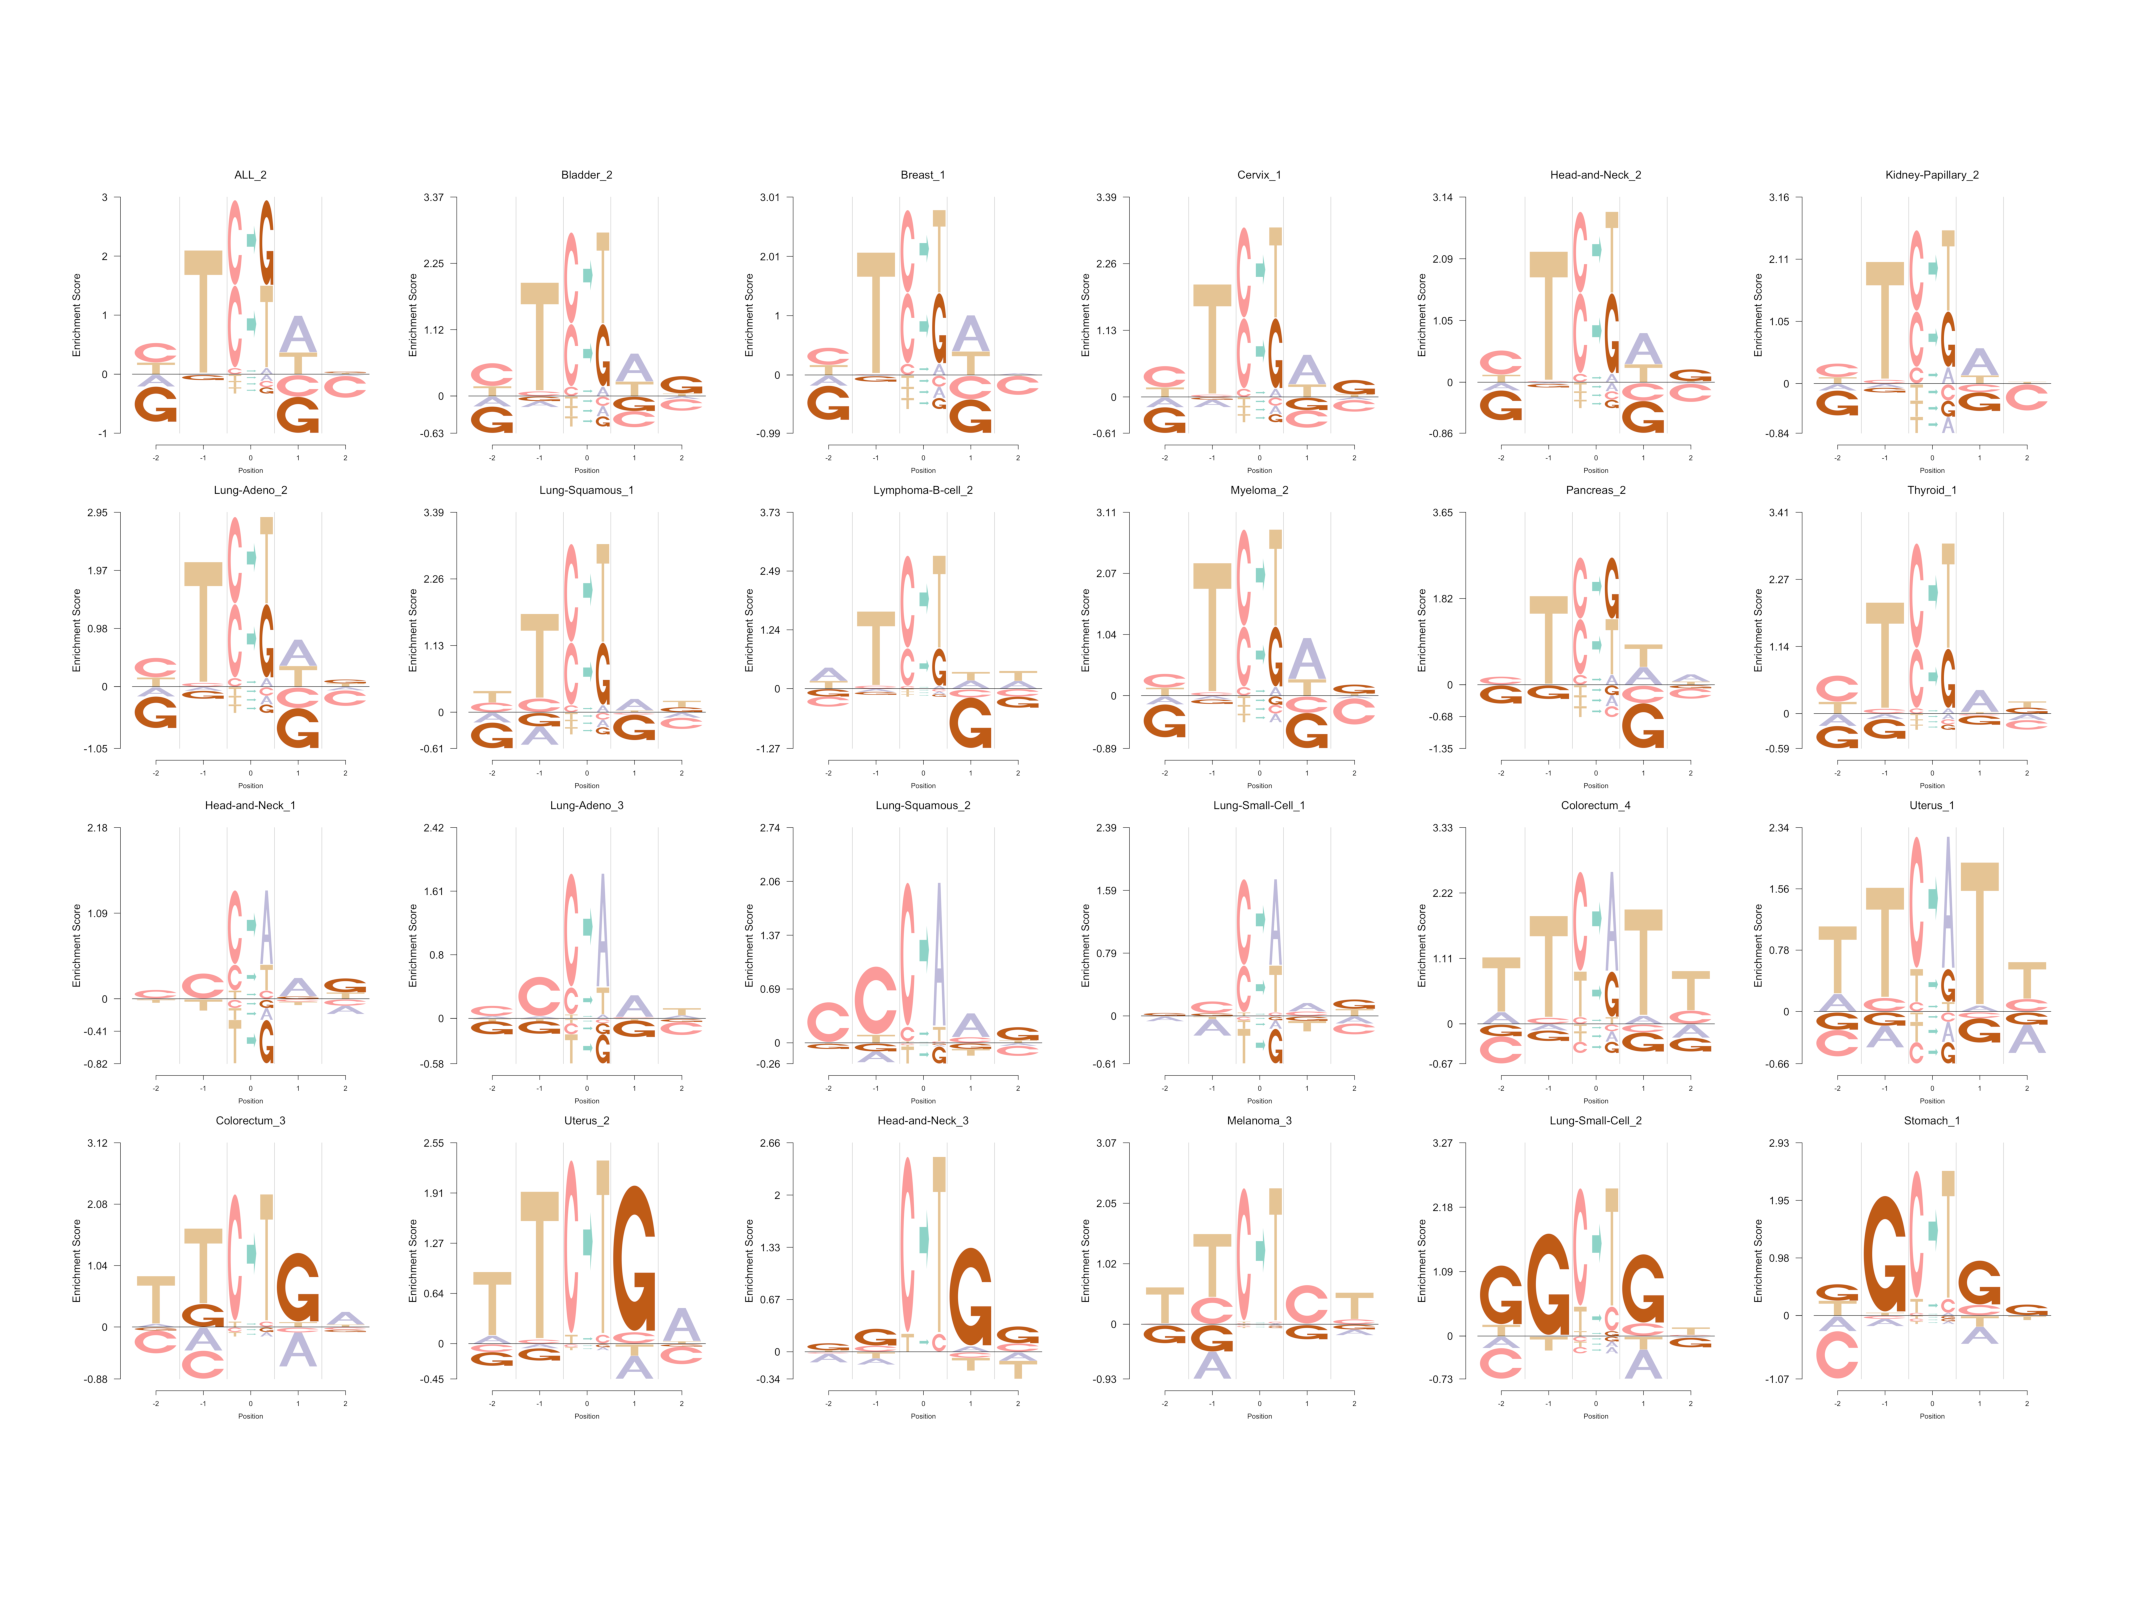
\includegraphics[height=6in, width=7in]{figures_folder/figures10.pdf}
\caption{\textbf{Logolas representation of cancer mutational signature profiles in alexandrov et al (2013).}
      We present the sparse logo representations of the cancer mutational signature profiles across a number of tissues where the mutational signature data has been  collected from 7042 cancers by Alexandrov et al (2013) \cite{Alexandrov2013}.  Each mutational signature profile has the mutation type at the center and is flanked by two bases to the left and two bases to the right.}
\label{fig:fig4}
\end{figure*}

\begin{figure*}[h!]
\centering
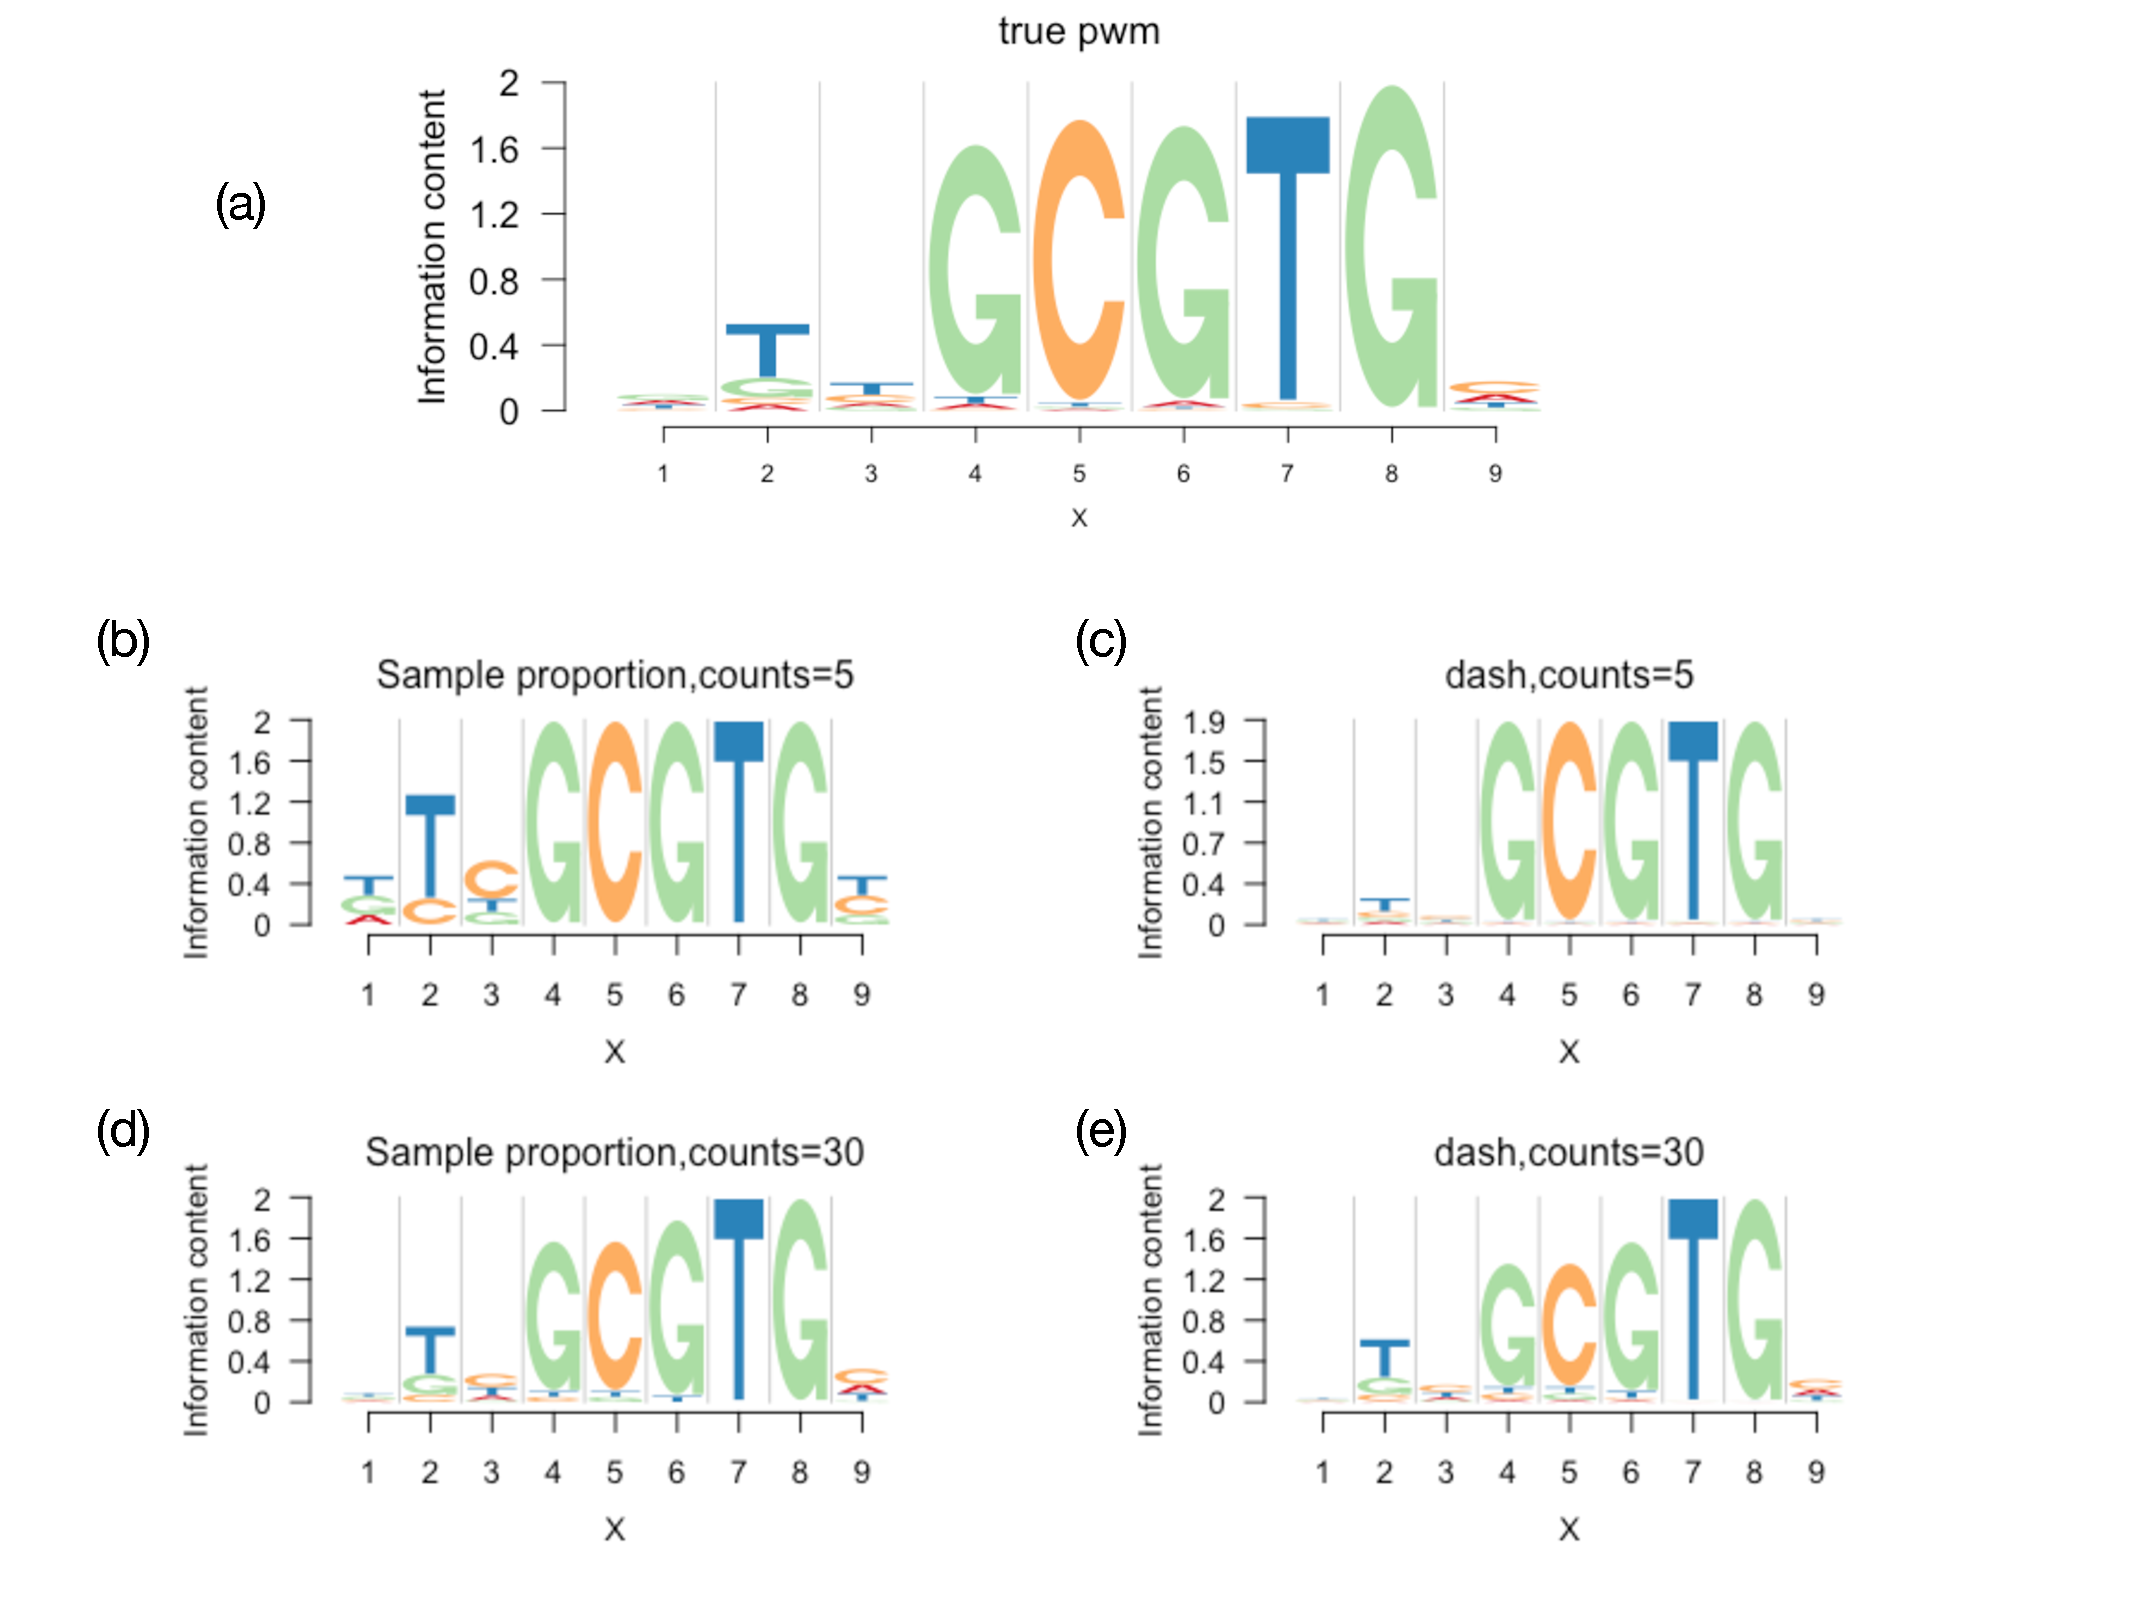
\includegraphics[height=6in, width=7in]{figures_folder/figures4.pdf}
\caption{\textbf{Subsampling experiment to validate the performance of Dirichlet Adaptive Shrinkage (dash).}
      In panel (a), we present the standard logo plot representation of the position frequency matrix (PFM) of the Aryl hydrocardon receptor. This PFM matrix is then used to define the position weights and two random subsamples, A of size 5 and B of size 30 are generated from this position weight matrix. Panels (b) and (c) demonstrate the logo plot representation estimated position weight matrix from the 5 symbols in the subsample A before applying dash and post dash scaling. Panels (d) and (e) show the same results for subsample B, with size 30. We notice that for subsample A case, the dash scaled PWM in panel (c) is a closer approximation of the original PWM in panel (a) compared to the pre-dash version in panel (b). However, the effect of dash is comparatively lower for subsample B, since the subsample size (30) is much larger and both the pre-dash and post-dash PWMs of subsampled symbols in panels (d) and (e) are good approximations to the original PWM.}
\label{fig:fig5}
\end{figure*}


\end{document}